
%% bare_conf.tex
%% V1.3
%% 2007/01/11
%% by Michael Shell
%% See:
%% http://www.michaelshell.org/
%% for current contact information.
%%
%% This is a skeleton file demonstrating the use of IEEEtran.cls
%% (requires IEEEtran.cls version 1.7 or later) with an IEEE conference paper.
%%
%% Support sites:
%% http://www.michaelshell.org/tex/ieeetran/
%% http://www.ctan.org/tex-archive/macros/latex/contrib/IEEEtran/
%% and
%% http://www.ieee.org/

%%*************************************************************************
%% Legal Notice:
%% This code is offered as-is without any warranty either expressed or
%% implied; without even the implied warranty of MERCHANTABILITY or
%% FITNESS FOR A PARTICULAR PURPOSE! 
%% User assumes all risk.
%% In no event shall IEEE or any contributor to this code be liable for
%% any damages or losses, including, but not limited to, incidental,
%% consequential, or any other damages, resulting from the use or misuse
%% of any information contained here.
%%
%% All comments are the opinions of their respective authors and are not
%% necessarily endorsed by the IEEE.
%%
%% This work is distributed under the LaTeX Project Public License (LPPL)
%% ( http://www.latex-project.org/ ) version 1.3, and may be freely used,
%% distributed and modified. A copy of the LPPL, version 1.3, is included
%% in the base LaTeX documentation of all distributions of LaTeX released
%% 2003/12/01 or later.
%% Retain all contribution notices and credits.
%% ** Modified files should be clearly indicated as such, including  **
%% ** renaming them and changing author support contact information. **
%%
%% File list of work: IEEEtran.cls, IEEEtran_HOWTO.pdf, bare_adv.tex,
%%                    bare_conf.tex, bare_jrnl.tex, bare_jrnl_compsoc.tex
%%*************************************************************************
\documentclass[9pt]{sig-alternate}

%\usepackage{biblatex}
%\usepackage{amsmath}
%\usepackage{amssymb}
%\usepackage{times}
\usepackage{hyperref}
%\usepackage{graphicx}
\usepackage{wrapfig}
\usepackage{listings}
\usepackage[usenames,dvipsnames]{xcolor}
%\usepackage{setspace}
\usepackage{python_syntax}
%\usepackage{bibentry}
\usepackage{todonotes}
\usepackage{url}
\usepackage{lineno}
%\usepackage{natbib}
%\usepackage{caption}
\usepackage[english]{babel} 
\def\UrlFont{\em} % Italicize all URLs.  
\lstset{
%	basicstyle=\tiny\ttfamily,
	breaklines=true,
	language=Python,
	}
\let\verbx\lstinline
\newcommand{\bfhead}[1]{\noindent \textbf{#1:}}

\usepackage{alltt}
\renewcommand{\ttdefault}{txtt}
%%\usepackage{color}
%%\usepackage[usenames,dvipsnames,svgnames,table]{xcolor}
%%\definecolor{mauve}{rgb}{0.58,0,0.82}
%\definecolor{light-gray}{gray}{0.75}
%\usepackage{listings}
%\lstset{
%  language=Python,
%  showstringspaces=false,
%  formfeed=\newpage,
%  tabsize=4,
%  commentstyle=\itshape,
%  basicstyle=\ttfamily\scriptsize,
%  morekeywords={lambda, self, assert, as},
%  numbers=left,
%  numberstyle=\scriptsize\color{light-gray}\textsf,
%  xleftmargin=2em,
%  stringstyle=\color{mauve}
%}
%\lstdefinestyle{Bash}{
%    language={}, 
%    moredelim=**[is][\color{blue}\bf\ttfamily]{`}{`},
%}
%\lstdefinestyle{OpenCL}{
%	language=C++,
%	morekeywords={kernel, __kernel, global, __global, size_t, get_global_id, sin}
%}
%
%\usepackage{float}
%\floatstyle{ruled}
%\newfloat{codelisting}{tp}{lop}
%\floatname{codelisting}{Listing}

% *** GRAPHICS RELATED PACKAGES ***
%
% *** MATH PACKAGES ***
%
%\usepackage[cmex10]{amsmath}
% A popular package from the American Mathematical Society that provides
% many useful and powerful commands for dealing with mathematics. If using
% it, be sure to load this package with the cmex10 option to ensure that
% only type 1 fonts will utilized at all point sizes. Without this option,
% it is possible that some math symbols, particularly those within
% footnotes, will be rendered in bitmap form which will result in a
% document that can not be IEEE Xplore compliant!
%
% Also, note that the amsmath package sets \interdisplaylinepenalty to 10000
% thus preventing page breaks from occurring within multiline equations. Use:
%\interdisplaylinepenalty=2500
% after loading amsmath to restore such page breaks as IEEEtran.cls normally
% does. amsmath.sty is already installed on most LaTeX systems. The latest
% version and documentation can be obtained at:
% http://www.ctan.org/tex-archive/macros/latex/required/amslatex/math/

% *** SPECIALIZED LIST PACKAGES ***
%
%\usepackage{algorithmic}
% algorithmic.sty was written by Peter Williams and Rogerio Brito.
% This package provides an algorithmic environment fo describing algorithms.
% You can use the algorithmic environment in-text or within a figure
% environment to provide for a floating algorithm. Do NOT use the algorithm
% floating environment provided by algorithm.sty (by the same authors) or
% algorithm2e.sty (by Christophe Fiorio) as IEEE does not use dedicated
% algorithm float types and packages that provide these will not provide
% correct IEEE style captions. The latest version and documentation of
% algorithmic.sty can be obtained at:
% http://www.ctan.org/tex-archive/macros/latex/contrib/algorithms/
% There is also a support site at:
% http://algorithms.berlios.de/index.html
% Also of interest may be the (relatively newer and more customizable)
% algorithmicx.sty package by Szasz Janos:
% http://www.ctan.org/tex-archive/macros/latex/contrib/algorithmicx/

% *** ALIGNMENT PACKAGES ***
%
%\usepackage{array}
% Frank Mittelbach's and David Carlisle's array.sty patches and improves
% the standard LaTeX2e array and tabular environments to provide better
% appearance and additional user controls. As the default LaTeX2e table
% generation code is lacking to the point of almost being broken with
% respect to the quality of the end results, all users are strongly
% advised to use an enhanced (at the very least that provided by array.sty)
% set of table tools. array.sty is already installed on most systems. The
% latest version and documentation can be obtained at:
% http://www.ctan.org/tex-archive/macros/latex/required/tools/

%\usepackage{mdwmath}
%\usepackage{mdwtab}
% Also highly recommended is Mark Wooding's extremely powerful MDW tools,
% especially mdwmath.sty and mdwtab.sty which are used to format equations
% and tables, respectively. The MDWtools set is already installed on most
% LaTeX systems. The lastest version and documentation is available at:
% http://www.ctan.org/tex-archive/macros/latex/contrib/mdwtools/

% IEEEtran contains the IEEEeqnarray family of commands that can be used to
% generate multiline equations as well as matrices, tables, etc., of high
% quality.

%\usepackage{eqparbox}
% Also of notable interest is Scott Pakin's eqparbox package for creating
% (automatically sized) equal width boxes - aka "natural width parboxes".
% Available at:
% http://www.ctan.org/tex-archive/macros/latex/contrib/eqparbox/

% *** SUBFIGURE PACKAGES ***
%\usepackage[tight,footnotesize]{subfigure}
% subfigure.sty was written by Steven Douglas Cochran. This package makes it
% easy to put subfigures in your figures. e.g., "Figure 1a and 1b". For IEEE
% work, it is a good idea to load it with the tight package option to reduce
% the amount of white space around the subfigures. subfigure.sty is already
% installed on most LaTeX systems. The latest version and documentation can
% be obtained at:
% http://www.ctan.org/tex-archive/obsolete/macros/latex/contrib/subfigure/
% subfigure.sty has been superceeded by subfig.sty.

%\usepackage[caption=false]{caption}
%\usepackage[font=footnotesize]{subfig}
% subfig.sty, also written by Steven Douglas Cochran, is the modern
% replacement for subfigure.sty. However, subfig.sty requires and
% automatically loads Axel Sommerfeldt's caption.sty which will override
% IEEEtran.cls handling of captions and this will result in nonIEEE style
% figure/table captions. To prevent this problem, be sure and preload
% caption.sty with its "caption=false" package option. This is will preserve
% IEEEtran.cls handing of captions. Version 1.3 (2005/06/28) and later 
% (recommended due to many improvements over 1.2) of subfig.sty supports
% the caption=false option directly:
%\usepackage[caption=false,font=footnotesize]{subfig}
%
% The latest version and documentation can be obtained at:
% http://www.ctan.org/tex-archive/macros/latex/contrib/subfig/
% The latest version and documentation of caption.sty can be obtained at:
% http://www.ctan.org/tex-archive/macros/latex/contrib/caption/

% *** FLOAT PACKAGES ***
%
%\usepackage{fixltx2e}
% fixltx2e, the successor to the earlier fix2col.sty, was written by
% Frank Mittelbach and David Carlisle. This package corrects a few problems
% in the LaTeX2e kernel, the most notable of which is that in current
% LaTeX2e releases, the ordering of single and double column floats is not
% guaranteed to be preserved. Thus, an unpatched LaTeX2e can allow a
% single column figure to be placed prior to an earlier double column
% figure. The latest version and documentation can be found at:
% http://www.ctan.org/tex-archive/macros/latex/base/

%\usepackage{stfloats}
% stfloats.sty was written by Sigitas Tolusis. This package gives LaTeX2e
% the ability to do double column floats at the bottom of the page as well
% as the top. (e.g., "\begin{figure*}[!b]" is not normally possible in
% LaTeX2e). It also provides a command:
%\fnbelowfloat
% to enable the placement of footnotes below bottom floats (the standard
% LaTeX2e kernel puts them above bottom floats). This is an invasive package
% which rewrites many portions of the LaTeX2e float routines. It may not work
% with other packages that modify the LaTeX2e float routines. The latest
% version and documentation can be obtained at:
% http://www.ctan.org/tex-archive/macros/latex/contrib/sttools/
% Documentation is contained in the stfloats.sty comments as well as in the
% presfull.pdf file. Do not use the stfloats baselinefloat ability as IEEE
% does not allow \baselineskip to stretch. Authors submitting work to the
% IEEE should note that IEEE rarely uses double column equations and
% that authors should try to avoid such use. Do not be tempted to use the
% cuted.sty or midfloat.sty packages (also by Sigitas Tolusis) as IEEE does
% not format its papers in such ways.

% *** PDF, URL AND HYPERLINK PACKAGES ***
%
% url.sty was written by Donald Arseneau. It provides better support for
% handling and breaking URLs. url.sty is already installed on most LaTeX
% systems. The latest version can be obtained at:
% http://www.ctan.org/tex-archive/macros/latex/contrib/misc/
% Read the url.sty source comments for usage information. Basically,
% \url{my_url_here}.

%\usepackage{placeins}

% *** Do not adjust lengths that control margins, column widths, etc. ***
% *** Do not use packages that alter fonts (such as pslatex).         ***
% There should be no need to do such things with IEEEtran.cls V1.6 and later.
% (Unless specifically asked to do so by the journal or conference you plan
% to submit to, of course. )


% correct bad hyphenation here
\hyphenation{op-tical net-works semi-conduc-tor}

\begin{document}
%
% paper title
% can use linebreaks \\ within to get better formatting as desired
\title{Collaborative Test-Driven Scientific Model Validation}


% author names and affiliations
% use a multiple column layout for up to two different
% affiliations
\numberofauthors{2}
\author{\alignauthor
Cyrus Omar, Jonathan Aldrich\\\affaddr{Carnegie Mellon University}\\
       \email{\{comar,aldrich\}@cs.cmu.edu}
       \alignauthor Richard C. Gerkin\\
       \affaddr{Arizona State University}\\{rgerkin@asu.edu}
}

% conference papers do not typically use \thanks and this command
% is locked out in conference mode. If really needed, such as for
% the acknowledgment of grants, issue a \IEEEoverridecommandlockouts
% after \documentclass

% for over three affiliations, or if they all won't fit within the width
% of the page, use this alternative format:
% 
%\author{\IEEEauthorblockN{Michael Shell\IEEEauthorrefmark{1},
%Homer Simpson\IEEEauthorrefmark{2},
%James Kirk\IEEEauthorrefmark{3}, 
%Montgomery Scott\IEEEauthorrefmark{3} and
%Eldon Tyrell\IEEEauthorrefmark{4}}
%\IEEEauthorblockA{\IEEEauthorrefmark{1}School of Electrical and Computer Engineering\\
%Georgia Institute of Technology,
%Atlanta, Georgia 30332--0250\\ Email: see http://www.michaelshell.org/contact.html}
%\IEEEauthorblockA{\IEEEauthorrefmark{2}Twentieth Century Fox, Springfield, USA\\
%Email: homer@thesimpsons.com}
%\IEEEauthorblockA{\IEEEauthorrefmark{3}Starfleet Academy, San Francisco, California 96678-2391\\
%Telephone: (800) 555--1212, Fax: (888) 555--1212}
%\IEEEauthorblockA{\IEEEauthorrefmark{4}Tyrell Inc., 123 Replicant Street, Los Angeles, California 90210--4321}}




% use for special paper notices
%\IEEEspecialpapernotice{(Invited Paper)}




% make the title area
\maketitle

\begin{abstract}
One of the pillars of the modern scientific method is \emph{model validation}: comparing a scientific model's predictions against empirical observations. Today, a scientist demonstrates the validity of a model by making an argument in a paper and submitting it for peer review, a process comparable to \emph{code review} in software engineering. While human review helps to ensure that contributions meet high-level goals, software engineers typically supplement this with \emph{unit testing} to get a more complete picture of the status of a software project, particularly for complex projects involving many developers. 

We argue that a similar test-driven methodology would be valuable to scientific communities as they seek to  validate increasingly complex models against growing collections of empirical data. The dynamics of  scientific communities and software communities differ in several key ways, however. In this paper, we introduce \emph{SciUnit}, a framework for test-driven scientific model validation. We describe how SciUnit, supported by new and existing collaborative infrastructure, can integrate into the modern scientific process.
%in the context of the applications and architectures that the language may need to target.
%
%Programming languages targeted toward end-users in high-performance computing must consider a number of issues in addition to performance. Typically, researchers have focused verifiability, portability and ease-of-use, and the right balance often depends on the particular uses that they are put toward.
%
%Ace %, evaluates it against several design and adoption criteria, and describes several use cases as well as a realistic case study involving parallelizing neurobiological circuit simulations on clusters of GPUs. 
%is an extensible statically-typed programming language embedded within the ubiquitous scripting language Python. Python serves as a {metalanguage}, enabling programmatic control over several aspects of language specification and compilation. 
%We demonstrate the power of this design for HPC by defining all of the primitives of the OpenCL kernel language as a library of user-defined types in Ace, then extending this core with several higher-level first-class abstractions. The target of translation, called the \emph{backend}, is user-defined as well, allowing us to implement the semantics of these primitives by direct translation to OpenCL, CUDA or C99.
%
%Although Ace is built around a static type discipline, it supports a novel form of generic programming based on type propagation that, together with a form of extensible local type inference, eliminates most of the syntactic overhead usually associated with statically-typed languages. A companion host API allows type information from \verb|numpy| arrays to directly propagate into Ace kernels, supporting seamless adoption of Ace into current scientific workflows.
%
\end{abstract}

%\begin{IEEEkeywords}
%extensible programming languages, heterogeneous computing, type systems
%\end{IEEEkeywords}


% For peer review papers, you can put extra information on the cover
% page as needed:
% \ifCLASSOPTIONpeerreview
% \begin{center} \bfseries EDICS Category: 3-BBND \end{center}
% \fi
%
% For peerreview papers, this IEEEtran command inserts a page break and
% creates the second title. It will be ignored for other modes.
%\IEEEpeerreviewmaketitle

\section{Introduction}
Scientific theories often take the form of a \emph{quantitative model}: a formal structure that can generate predictions about observable quantities. Such a model is characterized by its \textit{scope}: the set of observable quantities that the model can predict, and by its \textit{validity}: the extent to which its predictions agree with experimental observations of these quantities. 

Quantitative models are described and validated using a social process: the scientific publication system. For a model to be accepted by the scientific community, scientists must write a paper describing it and providing  evidence that it predicts some quantity of interest more accurately than previous models, or that the tradeoff it makes between accuracy and complexity may be useful to the community \cite{box}. During the \emph{peer review} process, other members of the relevant community are tasked with ensuring that the validation criteria used (e.g. a $p$-value) are strong enough and that all relevant data and competing models were fully considered, drawing on knowledge of statistical methods and the prior literature. Publishing a paper is one of the primary motivators for most scientists \cite{howison2011scientific}.

Quantitative scientific modeling and software development have much in common. Indeed, quantitative models are increasingly implemented as computer programs. In some cases, the program \emph{is} the model (e.g. complex simulations). The peer review process is similar in many ways to the \emph{code review} process used in many development teams. During code review, team members look for errors, enforce style and architectural guidelines and check that the code is \emph{valid} (i.e. that achieves its intended goal \cite{validity}) before it can be committed to the primary source code repository \cite{codereview}. 


Code review is reasonably effective \cite{creffectiveness1,creffectiveness2}. However, to be most effective reviewers must expend considerable effort \cite{effort}, and code review is most effective for resolving  issues related to software architecture \cite{evolvability}. 
For these reasons, most software development teams supplement code reviews with a number of more {automated} approaches to verification and validation. One of the most widely-adopted approaches is \emph{unit testing}.

--------

However, in many areas, the number of publications being generated every year can overwhelm even the most conscientious scientists \cite{jinha_article_2010}. 

%This suggests that tools that help researchers answer questions like these could help readers and reviewers develop a more comprehensive understanding of the state-of-the-art and improve the quality of the research being published as a result: to renewed calls for tools that help researchers . 

Unfortunately, there are few alternatives to a comprehensive literature review available when scientists need to answer questions like these:
\begin{itemize}
\item Which models are capable of predicting the quantities I am interested in?
\item Which metrics should be used to evaluate the goodness-of-fit between these models and  data?
\item How well do these models perform, as judged to these metrics, given currently available data?
\item What other quantities can and can't these models predict?
\item What observations are not adequately explained by any available model?
\end{itemize}

%These questions are particularly relevant for young scientists and  scientists aiming to enter a new research area to answer.

%understanding of the state-of-the-art from publications containing only a few pieces of data, and then only that data available at the time of publication. 

%These demonstrations also quickly go out of date. Finally, there is no easy way to summarize and compare the claims being made in modeling papers in order to synthesize an understanding of a research area as a whole. 
%A strength of publications are their focused descriptions of new data and models. 
%A weakness, however, is that evaluating the scope and validity of models against known data is intractable using a body of publications alone.

Professional software developers face similar issues. 
They must understand the scope of each component of a complex software project and validate it by measuring how well each component achieves its specified input/output behavior. 
But software developers do not validate components by simply choosing a few interesting inputs and presenting the outputs to reviewers. 
Rather, they typically follow a \emph{test-driven development} methodology by creating a suite of executable \emph{unit tests} that serve to specify each component's scope and validate its implementation as it is being developed and modified \cite{beck2003}. 
Each test individually checks that a small portion of the program meets a single correctness criterion. For example, a unit test might verify that one function within the program correctly handles malformed inputs. 
Collectively, the test results serve as a summary of the validity of the project as it progresses through its development cycle. 
Developers can determine which features are unimplemented or buggy by examining the set of failed tests, and progress can be measured in terms of how many tests the program passes over time. 
This methodology is widely adopted in practice \cite{beck2003}.

%publications would be analagous to user manuals, rather than rigorous justifications that a program meets a specific specification. Unit tests serve this purpose for software, so we argue that the validation of neuroscience models by means of executable tests would be useful to scientists as a supplement the publication system.

Test-driven methodologies have started to see success in neuroscience as well. 
Modeling competitions in neuroscience, for example, are typically organized around a collection of simple validation criteria, implemented as executable tests. 
These competitions continue to drive important advances and improve scientists' understanding of the relative merits of different models. 
For example, the quantitative single neuron modeling competition (QSNMC) \cite{jolivet_quantitative_2008} investigates the complexity-accuracy tradeoff among reduced models of excitable membranes; 
the ``Hopfield'' challenge \cite{hopfield_what_2000} tested techniques for generating neuronal network form given its function; 
the Neural Prediction Challenge sought the best stimulus reconstructions, given neuronal activity (\url{http://neuralprediction.berkeley.edu}); the Diadem challenge is advancing the art of neurite reconstruction (\url{http://www.diademchallenge.org}); and 
examples from other subfields of biology abound (\url{http://www.the-dream-project.org}).
% \begin{figure}%{r}{0.6\textwidth}
% %\vspace{-38px}
% \includegraphics[scale=0.75]{sciunit_overview.pdf}
% \caption{Proposal overview. 
% \small{i) The \textit{SciUnit} framework can generate discipline-specific libraries for tests generation and model interfacing.  
% \textit{NeuronUnit} is proposed and described here.  Experimental data guides test development; model generation informs and is informed by these \textit{SciUnit} libraries.  
% Each \text{SciUnit} test suite repository on GitHub is indexed by the \textit{SciDash} web application.  
% Test suites for OSB and QSNMC (described in the text) are being built. 
% \textit{SciDash} automatically runs the test collections in each suite and publicly displays the results.}}
% %\vspace{-10px}
% \label{fig:sciunit_overview}
% \end{figure}
% \leavevmode
% \vspace{-0px}
\begin{figure*}[t]
\centering
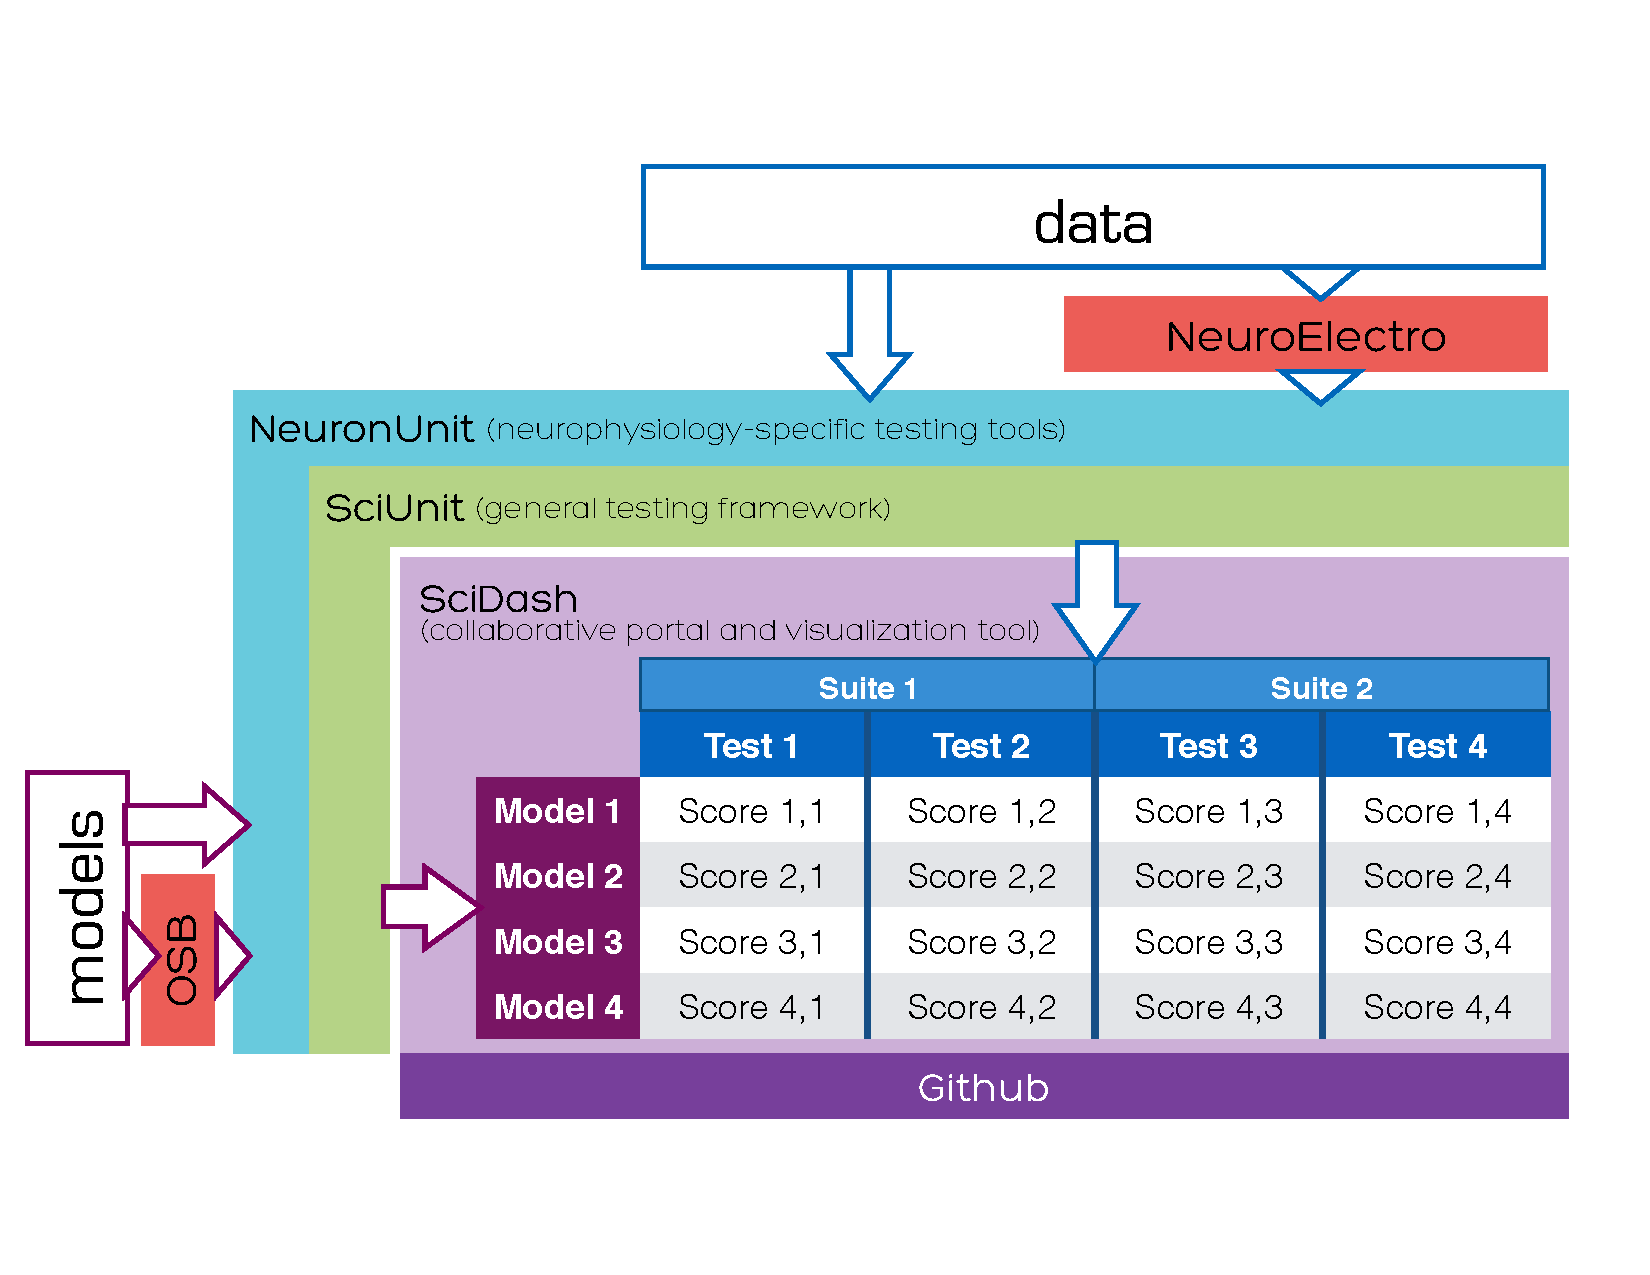
\includegraphics[scale=0.4]{diagram1.pdf}
\vspace{-25px}
\caption{NeuronUnit overview. NeuronUnit is set of testing tools built upon the discipline-agnostic SciUnit framework. 
NeuronUnit can in principle test arbitrary neurophysiology models using arbitrary data but we provide here an example using models described in NeuroML as part of the \textit{Open Source Brain Project} (OSB, \cite{gleeson_open_2012}, \url{http://www.opensourcebrain.org}), and single neuron electrophysiology data available as part of the NeuroElectro Project (Neuroelectro, \cite{tripathy_neuroelectro:_2012}, \url{http://neuroelectro.org}).  
Records of test results for various model/test combinations are accessible via SciDash, which indexes GitHub repositories of these records, models, and tests so they can be searched and filtered by the community.}  
\label{fig:sciunit_overview}
\end{figure*}
\leavevmode
\vspace{-0px}

Each of these examples has leveraged \emph{ad hoc} infrastructure to support test generation. 
While the specific criteria used to evaluate models varies widely between disciplines in neuroscience, the underlying test-driven methodology has many common features that could be implemented once. 
Recognizing this, we developed a discipline-agnostic framework for developing scientific validation test suites called \textit{SciUnit} (\url{http://www.sciunit.org}). 
Here we describe \textit{NeuronUnit\-}, which builds upon \textit{SciUnit}, allowing neuroscientists to build \textit{SciUnit} tests that validate neurophysiology models against electrophysiological data.  We provide a concrete example pipeline, showing how models described using \text{NeuroML} and provided freely by the \textit{Open Source Brain Project} (OSB, \cite{gleeson_open_2012}, \url{http://www.opensourcebrain.org}) can be tested in fully automated fashion using published, curated data available through the \textit{NeuroElectro Project} (Neuroelectro, \cite{tripathy_neuroelectro:_2012}, \url{http://neuroelectro.org}), leveraging facilities from the \textit{NeuroTools} library (\url{http://neuralensemble.org/NeuroTools}) to extract relevant features of model output.  This is summarized in Figure \ref{fig:sciunit_overview}, which shows the relationships between the layers described here.
% In addition to this open testing toolkit we also provide a library of tests for models of spiking single neurons.  

% Section 2.
\section{Validation Testing with \textit{SciUnit}}
\subsection{Example: The Quantitative Single Neuron Modeling Competition}
\begin{figure}[t]
\small
\begin{python}
class SpikeCountTest(sciunit.Test):
  """Tests spike counts produced in response to several current stimuli against observed means and standard deviations. 

  goodness of fit metric: Computes p-values based on a chi-squared test statistic, and pools them using Fisher's method.
  parameters:
    inputs: list of numpy arrays containing input currents (nA)
    means, stds: lists of observed means and standard deviations, one per input
  """
  def __init__(self, inputs, means, stds):
    self.inputs, self.means, self.stds = inputs, means, stds
	
  required_capabilities = [SpikeCountFromCurrent]
	
  def _judge(self, model):
    inputs, means, stds = self.inputs, self.means, self.stds
    n = len(inputs)
    counts = numpy.empty((n,))
    for i in xrange(n):
      counts[i] = model.spike_count_from_current(inputs[i])
    chisquared = sum((counts-means)**2 / means) # An array of chi-squared values.  
    p = scipy.stats.chi2.cdf(chisquared,n-1) # An array of p-values.  
    pooled_p = sciunit.utils.fisherp(p_array) # A pooled p-value.  
    return sciunit.PValue(pooled_p, related_data={
      "inputs": inputs, "counts": counts, "obs_means": means, "obs_stds": stds
    })
\end{python}
\vspace{-5px}
\caption{An example single neuron spike count test class implemented using \textit{SciUnit}. Because this implementation contains logic common to many different systems, \textit{NeuronUnit} was developed to provide a simpler means to deliver it (see Sec. \ref{sec:neuronunit}).}
\label{fig:rate_test}
\vspace{-15px}
\end{figure}

%Simple executable \emph{validation tests} that compute agreement between a model prediction and an experimental observation.  
We first illustrate the form of a generic example \textit{SciUnit} test suite that could be used in neurophysiology. 
Suppose we have collected data from an experiment where current stimuli (measured in pA) are delivered to neurons in some brain region, while the somatic membrane potential of each stimulated cell (in mV) is recorded and stored.  
A model claiming to capture this cell type's membrane potential dynamics must be able to accurately predict a variety of features observed in these data.

One simple validation test would ask candidate models to predict the number of action potentials (a.k.a. spikes) generated in response to a stimulus (e.g. white noise), and compare these \emph{spike count} predictions to the distribution observed in repeated experimental trials using the same stimulus. 
For data of this type, goodness-of-fit can be measured by first calculating a p-value from a chi-squared statistic for each prediction and then combining these p-values using Fisher's method \cite{fisher_statistical_1925}. 

Alongside this \emph{spike count test}, we might also specify a number of other tests capturing different features of the data  to produce a more comprehensive suite. 
For data of this sort, the QSNMC defined 17 other validation criteria in addition to one based on the overall spike count, capturing features like spike latencies (SL), mean subthreshold voltage (SV), interspike intervals (ISI) and interspike minima (ISM) that can be extracted from the data \cite{jolivet_quantitative_2008}. 
They then defined a combined metric favoring models that broadly succeeded at meeting these criteria, to produce an overall ranking. 
Such combined criteria are simply validation tests that invoke other tests to produce a result.
 
%In many cases, models require no modifications to take the new tests because the same type of model output is being requested.
\subsection{Implementing a Validation Test in \textit{SciUnit}}
Fig. \ref{fig:rate_test} shows how a scientist can implement spike count tests such as the one described above using \textit{SciUnit}. 
A \textit{SciUnit} validation test is an {instance} (i.e. an object) of a Python class implementing the \verbx{sciunit.Test} interface (cf. line 1). 
Here, we show a class \verbx{SpikeCountTest} taking three \emph{parameters} in its constructor (constructors are named \verbx{__init__} in Python, lines 9-10). 
The meaning of each parameter along with a description of the goodness-of-fit metric used by the test is documented on lines 4-7. 
%For convenience, we also make use of functions provided by the popular NumPy\cite{numpy_url} and SciPy\cite{scipy_url} libraries, although these are not required by \textit{SciUnit}.  
To create a \emph{particular} spike count test, we instantiate this class with particular experimental observations. 
For example, given observations from hippocampal CA1 cells (not shown), we can instantiate a test as follows:
\begin{python}
  CA1_sc_test = SpikeCountTest(CA1_inputs, CA1_means, CA1_stds)
\end{python}
We emphasize the crucial distinction between the \textit{class} \verbx{SpikeCountTest}, which defines a \emph{parameterized family} of validation tests, and the particular \textit{instance} \verbx{CA1_sc_test}, which is an individual validation test because the necessary parameters, derived from data, have been provided. 
As we will describe below, we expect communities to build repositories of such families capturing the criteria used in their subfields of neuroscience so that test generation for a particular system of interest will often require simply instantiating a previously-developed family with particular experimental parameters and data. 
For single-neuron test families like \verbx{SpikeCountTest}, we have developed such a library, called \textit{NeuronUnit} (\url{http://github.com/scidash/neuronunit}) (Sec. \ref{sec:neuronunit}). 

Classes that implement the \verbx{sciunit.Test} interface must contain a \verbx{_judge} method that receives a candidate \emph{model} as input and produces a \textit{score} as output. 
To specify the interface between the test and the model (that is, to specify an appropriate scope), the test author provides a list of \emph{capabilities} in the \verbx{required_capabilities} attribute, seen on line 12 of Fig. \ref{fig:rate_test}. 
Capabilities are simply collections of methods that a test will need to invoke in order to receive relevant data, and are analogous to \emph{interfaces} in e.g. Java (\url{http://docs.oracle.com/javase/tutorial/java/concepts/interface.html}). 
In Python, capabilities are written as classes with unimplemented members. 
The capability required by the test in Fig. \ref{fig:rate_test} is shown in Fig. \ref{fig:capability}. 
In \textit{SciUnit}, classes defining capabilities are tagged as such by inheriting from \verbx{sciunit.Capability}. The test in Figure \ref{fig:rate_test} uses this capability on line 19 to produce a spike count prediction for each input current. 

The remainder of the \verbx{_judge} method implements the goodness-of-fit metric described above, returning an instance of \verbx{sciunit.PValue}, a subclass of \verbx{sciunit.Score} that is included with \textit{SciUnit}. In addition to the $p$-value itself, the returned score object also contains metadata, via the \verbx{related_data} parameter, for  scientists who may wish to examine the result in more detail later. 
In this case we save the input currents, the model outputs and the observed means and standard deviations (line 24). 
%We discuss visualization of results in Secs. \ref{sec:scidash_activities} and \ref{sec:scidash_visualization}.

\begin{figure}
\begin{python}
class SpikeCountFromCurrent(sciunit.Capability):
  def spike_count_from_current(self, input): 
    """Takes a numpy array containing current stimulus (in nA) and
    produces an integer spike count. Can be called multiple times."""
    raise NotImplementedError("Model does not implement capability.")
\end{python}
\caption{An example capability specifying a single required method (used by the test in Figure \ref{fig:rate_test}).}
\label{fig:capability}
\vspace{-10px}
\end{figure}

\begin{figure}
\begin{python}
class TrainSpikeCountFromCurrent(sciunit.Capability):
  def train_with_currents(self, currents, counts):
    """Takes a list of numpy arrays containing current stimulus (in nA) and
    observed spike counts. Model parameters should be adjusted based on this
    training data."""
    raise NotImplementedError("Model does not implement capability.")
\end{python}
\caption{Another capability specifying a training protocol (not used by the test in Figure \ref{fig:rate_test}).}
\label{fig:training}
\vspace{-15px}
\end{figure}

\subsection{Models}
Capabilities are \emph{implemented} by models. In \textit{SciUnit}, models are instances of Python classes that inherit from \verbx{sciunit.Model}. Like tests, the class itself represents a family of models, parameterized by the arguments of the constructor. A particular model is an instance of such a class.

Figure \ref{fig:simple_model} shows how to write a simple {family} of models, \verbx{LinearModel}, that implement the capability in Fig. \ref{fig:capability} as well as another capability shown in Fig. \ref{fig:training}, which we will discuss below. 
Models in this family generate a spike count by applying a linear transformation to the mean of the provided input current. The family is parameterized by the scale factor and the offset of the transformation, both scalars. 
To create a \emph{particular} linear model, a modeler can provide particular parameter values, just as with test families:
\begin{python}
CA1_linear_model_heuristic = LinearModel(3.0, 1.0)
\end{python}
Here, the parameters to the model were picked by the modeler heuristically, or based on externally-available knowledge. 
An alternative test design would add a training phase where these parameters were fit to data using the capability shown in Fig. \ref{fig:training}. 
This test could thus only be used for those models for which parameters can be adjusted without human involvement. 
Whether to build a training phase into the test protocol is a choice left to each test development community. 

Fig. \ref{fig:rate_test} does not include a training phase. 
If training data is externally available, models that nevertheless do implement a training capability (like \verb|LinearModel|) can simply be trained explicitly by calling the capability method just like any other Python method:
\begin{python}
CA1_linear_model_fit = LinearModel()
CA1_linear_model_fit.train_with_currents(CA1_training_in, CA1_training_out)
\end{python}
\begin{figure}
\begin{python}
class LinearModel(sciunit.Model, SpikeCountFromCurrent, 
    TrainSpikeCountFromCurrent):
  def __init__(self, scale=None, offset=None): 
    self.scale, self.offset = scale, offset
    
  def spike_count_from_current(self, input):
    return int(self.scale*numpy.mean(input) + self.offset)

  def train_with_currents(self, currents, counts):
    means = [numpy.mean(c) for c in currents]
    [self.offset, self.scale] = numpy.polyfit(means, counts, deg=1)    
\end{python}
\caption{A model that returns a spike count by applying a linear transformation to the mean input current. The parameters can be provided manually or learned from data provided by a test or user (see text).}
\label{fig:simple_model}
\vspace{-15px}
\end{figure}

\subsection{Executing Tests} A test is executed against a model using the \verbx{judge} method:
\begin{python}
score = CA1_sc_test.judge(CA1_linear_model_heuristic)
\end{python}

This method proceeds by first checking that the provided model implements all required capabilities. It then calls the test's \verbx{_judge} method to produce a score. A reference to the test and model are added to the score for convenience (accessible via the \verbx{test} and \verbx{model} attributes, respectively), before it is returned.

\subsection{Test Suites and Score Matrices} A collection of tests intended to be run on the same model can be put together to form a test suite.
The following is a test suite that could be used for a simplified version of the QSNMC, as described above:  
\begin{python}
CA1_suite = sciunit.TestSuite([CA1_sc_test, CA1_sl_test, CA1_sv_test, CA1_isi_test, CA1_ism_test])
\end{python}
Like a single test, a test suite is capable of judging one or more models. The result is a score matrix much like the one diagramed in Fig. \ref{fig:sciunit_overview}.
\begin{python}
CA1_matrix = CA1_suite.judge([CA1_linear_model_heuristic, CA1_linear_model_fit])
\end{python}
A simple summary of the scores in a score matrix can be printed to the console or  visualized by other tools, such as the web application \textit{SciDash} described in Sec. \ref{sec:scidash}.



% conference papers do not normally have an appendix


% use section* for acknowledgement
% trigger a \newpage just before the given reference
% number - used to balance the columns on the last page
% adjust value as needed - may need to be readjusted if
% the document is modified later
%\IEEEtriggeratref{8}
% The "triggered" command can be changed if desired:
%\IEEEtriggercmd{\enlargethispage{-5in}}

% references section

% can use a bibliography generated by BibTeX as a .bbl file
% BibTeX documentation can be easily obtained at:
% http://www.ctan.org/tex-archive/biblio/bibtex/contrib/doc/
% The IEEEtran BibTeX style support page is at:
% http://www.michaelshell.org/tex/ieeetran/bibtex/
%\bibliographystyle{IEEEtran}
% argument is your BibTeX string definitions and bibliography database(s)
%\bibliography{IEEEabrv,../bib/paper}
%
% <OR> manually copy in the resultant .bbl file
% set second argument of \begin to the number of references
% (used to reserve space for the reference number labels box)
\bibliographystyle{IEEEtran}
\bibliography{../research}
%
%\begin{thebibliography}{1}
%
%\bibitem{IEEEhowto:kopka}
%H.~Kopka and P.~W. Daly, \emph{A Guide to \LaTeX}, 3rd~ed.\hskip 1em plus
%  0.5em minus 0.4em\relax Harlow, England: Addison-Wesley, 1999.
%
%\end{thebibliography}




% that's all folks
\end{document}


